%\section{Resultados}
\chapter{Resultados e Discussões}
\label{sec:result}
\index{Métodos e Resultados!Resultados}
Esta seção apresenta os resultados e discute as técnicas de \textit{bootstrap}, \textit{bagging} e \textit{subagging} aplicadas à regressão linear múltipla. Ela avalia o erro médio quadrático de predição (RMSEP) e compara os tempos de execução dos algoritmos RLM, RLM-\textit{bagging} e RLM-\textit{subagging}.

\def\namostras{Nº de amostras}


\begin{table}[!htbp]
\centering
\small
\begin{threeparttable}
\caption{RMSEP por analito obtido via RLM para amostras de aço-ligas.}
\label{tab:rmseprlm}
\begin{tabular}{p{3cm} p{4cm}} % Define larguras fixas
%\begin{tabular}{lc} % Duas colunas apenas
\toprule
\textbf{Elementos} & \textbf{RMSEP (RLM)} \\ 
\midrule
Mn & \num{\dados[2,2]} \\ 
Mo & \num{\dados[2,3]} \\ 
Cr & \num{\dados[2,4]} \\ 
Ni & \num{\dados[2,5]} \\ 
Fe & \num{\dados[2,6]} \\ 
\bottomrule
\end{tabular}
\begin{tablenotes}[flushleft] % Garante o alinhamento exatamente abaixo do analito
    \footnotesize
    \item \footnotesize Fonte:~\oautor
\end{tablenotes}
\end{threeparttable}
\end{table}

A Tabela~\ref{tab:rmseprlm} mostra o RMSEP obtido com a RLM para todas as amostras de aço-ligas.
%-------------------SubFigure

\begin{figure}[htbp]
\centering
\caption{RMSEP com RLM para Mn e Fe.}
\label{fig:Figura41} % Main figure label

% Gráfico da esquerda (Mn)
\begin{subfigure}{0.48\textwidth}
\centering
\begin{tikzpicture}
    \begin{axis}[
        xlabel=\namostras,
        ylabel=Concentrações,
        %title=(a) RMSEP com RLM para o Mn,
        legend style={
            at={(0.5,1.05)}, % Posição acima do gráfico
            anchor=south, % Âncora no sul (parte de baixo da legenda)
            legend columns=2, % Duas colunas para legenda compacta
            font=\footnotesize
        },
        grid=major,
        width=\textwidth
    ]
    \addplot[mark=none, color=red] table[x index=0, y index=1, col sep=space] {tex/YtesteMn.txt};
    \addplot[mark=none, color=blue] table[x index=0, y index=1, col sep=space] {tex/CpredMn.txt};
    \legend{Conc. pred., Conc. ref.}
    \end{axis}
\end{tikzpicture}
\caption{RMSEP com RLM para Mn.}
\label{fig:Figura41a} % Left subfigure label
\end{subfigure}
\hfill
% Gráfico da direita (Fe)
\begin{subfigure}{0.48\textwidth}
\centering
\begin{tikzpicture}
    \begin{axis}[
        xlabel=\namostras,
        ylabel=Concentrações,
        %title=(b) RMSEP com RLM para o Fe,
        legend style={
            at={(0.5,1.05)}, % Posição acima do gráfico
            anchor=south, % Âncora no sul (parte de baixo da legenda)
            legend columns=2, % Duas colunas para legenda compacta
            font=\footnotesize
        },
        grid=major,
        width=\textwidth
    ]
    \addplot[mark=none, color=red] table[x index=0, y index=1, col sep=space] {tex/YtesteFe.txt};
    \addplot[mark=none, color=blue] table[x index=0, y index=1, col sep=space] {tex/CpredFe.txt};
    \legend{Conc. pred., Conc. ref.}
    \end{axis}
\end{tikzpicture}
\caption{RMSEP com RLM para Fe.}
\label{fig:Figura41b} % Right subfigure label
\end{subfigure}

\legend{\footnotesize Fonte:~\oautor}
\end{figure}
%-----------------Subfigure

A Figura~\ref{fig:Figura41} exibe o comportamento do RMSEP para os elementos Mn e Fe. A Figura~\ref{fig:Figura41a} detalha o RMSEP do manganês (Mn) e a Figura~\ref{fig:Figura41b}, o do ferro (Fe). O sinal azul representa a concentração esperada do Mn e do Fe e sinal vermelho a concentração predita obtida com a RLM. Pode ser visto na Tabela~\ref{tab:rmseprlm} que o Mn apresenta o menor RMSEP entre os três métodos, com destaque para o RLM-\textit{subagging}~(\num{0,0974}). Por outro lado, o Fe apresenta o maior RMSEP, com o valor mais elevado obtido pela RLM~(\num{2,7513}). De forma geral, o RLM-\textit{subagging} apresentou desempenho superior ao RLM-\textit{bagging} na maioria dos elementos analisados, embora a RLM clássica tenha se mantido como método de menor RMSEP para Mo e Cr, indicando que a técnica mais adequada depende das características específicas de cada analito.

A escolha dos elementos ferro e manganês para esta análise baseia-se em fundamentos científicos bem estabelecidos na metalurgia. O ferro é o elemento matriz que define a própria natureza do material, uma vez que sem ferro não existe aço. O manganês, por sua vez, é o único elemento de liga historicamente considerado essencial para a produção de qualquer aço comercial, atuando como desoxidante e modificador fundamental das propriedades mecânicas. Os demais elementos (Cr, Mo, Ni) são importantes para propriedades específicas, mas não são fundamentais para a definição básica e produção do aço como o ferro e o manganês. Acredita-se que o comportamento destas duas amostras são suficientes para ilustrar o comportamento geral esperado para as outras amostras.


%----------------------------------------------------------------------------------------------------------
\section{\textit{Bagging}}
\label{sec:bagging2}
\index{Métodos e Resultados!\textit{Bagging}}
Os resultados obtidos com a técnica \textit{bagging} foram produzidos com a implementação do Algoritmo~\ref{alg:bagging}. Contudo, como visto na Subseção~\ref{sec:bagging} da Seção~\ref{sec:teclarea}, o algoritmo RLM-\textit{bagging} depende do parâmetro $m$ que define o número de replicações \textit{bootstrap}.

Foi conduzido um experimento para avaliar a sensibilidade do \textit{bagging} em função do número de replicações, variando de 1 a 50. O procedimento experimental implementou o RLM-\textit{bagging} com um algoritmo iterativo que modifica sistematicamente o número de replicações utilizadas.

%------------------------------------------------------------------------------------------------
\begin{figure}[htbp]
\centering
\caption{RMSEP em função do número de replicações \textit{bootstrap} para RLM-\textit{bagging}.}
\label{fig:Figura42} % Main figure label
% Gráfico da esquerda (Mn)
\begin{subfigure}{0.48\textwidth}
\centering
\begin{tikzpicture}
    \begin{axis}[
        xlabel=Número de replicações,
        ylabel=RMSEP,
        %title=RMSEP com RLM-bagging para o Mn,
        legend pos=north east,
        grid=major,
        width=\textwidth
    ]
    \addplot[mark=none,line width=1.0pt,color=blue] table[x index=0, y index=1, col sep=space] {tex/bagging_mn.txt};
    \addplot[only marks, mark=*, mark size=2pt, color=red] coordinates {(28,0.0253885541)};
    \node at (axis cs:28,0.0253885541) [anchor=south west, color=red] {\scriptsize(28,\ 0.025)};
    %\addplot[mark=none, color=blue] table[x index=0, y index=1, col sep=space] {tex/CpredMn.txt\node at (axis cs:56,0.102871) [anchor=south west, color=red] {\scriptsize(56,\ 0.102)};};
    %\legend{Conc. pred., Conc. espe.}
    \end{axis}
\end{tikzpicture}
\caption{RMSEP em função do número de replicação para o Mn.}
\label{fig:Figura42a} % Left subfigure label
\end{subfigure}
\hfill
% Gráfico da direita (Fe)
\begin{subfigure}{0.48\textwidth}
\centering
\begin{tikzpicture}
    \begin{axis}[
        xlabel=Número de replicações,
        ylabel=RMSEP,
        %title=RMSEP com RLM-bagging para o Fe,
        legend pos=north east,
        grid=major,
        width=\textwidth
    ]
    \addplot[mark=none,line width=1.0pt ,color=blue] table[x index=0, y index=1, col sep=space] {tex/bagging_fe.txt};
    \addplot[only marks, mark=*, mark size=2pt, color=red] coordinates {(3,1.3282)};
    \node at (axis cs:3,1.3282) [anchor=north west, color=red] {\scriptsize(3,\ 1.328)};
    %\addplot[mark=none, color=blue] table[x index=0, y index=1, col sep=space] {tex/CpredFe.txt};
    %\legend{Conc. pred., Conc. espe.}
    \end{axis}
\end{tikzpicture}
\caption{RMSEP em função do número de replicação para o Fe.}
\label{fig:Figura42b} % Right subfigure label
\end{subfigure}
\legend{\footnotesize Fonte:~\oautor}
\end{figure}

%-------------------------------------------------------------------------------------------------------
A Figura~\ref{fig:Figura42} mostra o RMSEP da RLM em função das replicações \textit{bootstrap}. A Figura~\ref{fig:Figura42a} mostra o comportamento do RLM-\textit{bagging} para o Mn e a Figura~\ref{fig:Figura42b} mostra o RMSEP do RLM-\textit{bagging} para o Fe.
Para o Manganês, observa-se comportamento mais estável após $(15-20)$ replicações, os valores do RMSEP tendem a se estabilizar em torno de $(0,026-0,030)$ e apresenta menor variabilidade absoluta. Para o Ferro, verifica-se maior oscilação ao longo de todas as replicações, os valores oscilam entre $(1,3-2,2)$ sem clara estabilização, apresentando maior variabilidade tanto absoluta quanto relativa. Existe considerável variabilidade para ambos os elementos, mas: o Ferro evidenciou a maior amplitude de variação entre os métodos, com desempenho variando de $34\%$ a $41\%$, indicando sensibilidade elevada à técnica utilizada. O Manganês apresenta tendência de estabilização após aproximadamente 20 replicações. O Ferro mantém oscilações mesmo com 50 replicações. Isso sugere que o \textit{bagging} para Fe pode precisar de mais replicações ou que a predição do Fe é inerentemente mais difícil que a do Mn. Os valores apresentados na Figura 6 foram obtidos com o conjunto de calibração completo utilizado internamente para análise de sensibilidade, podendo diferir dos valores do conjunto de teste independente reportados nas Tabelas 5 e 9.

\begin{figure}[!htbp]
\centering
\caption{RMSEP para o Mn e Fe com RLM-\textit{bagging}.}
\label{fig:Figura43} % Main figure label

% Gráfico da esquerda (Mn)
\begin{subfigure}{0.48\textwidth}
\centering
\begin{tikzpicture}
    \begin{axis}[
        xlabel=\namostras,
        ylabel=Concentrações,
        %title=RMSEP com RLM-bagging para o Mn,
        legend style={
            at={(0.5,1.05)}, % Posição acima do gráfico
            anchor=south, % Âncora no sul (parte de baixo da legenda)
            legend columns=2, % Duas colunas para legenda compacta
            font=\footnotesize
        },
        grid=major,
        width=\textwidth
    ]
    \addplot[mark=none, color=red] table[x index=0, y index=1, col sep=space] {tex/YtesteMn.txt};
    \addplot[mark=none, color=blue] table[x index=0, y index=1, col sep=space] {tex/CpredMn.txt};
    \legend{Conc. pred., Conc. ref.}
    \end{axis}
\end{tikzpicture}
\caption{Predição do Mn com RLM-\textit{bagging}.}
\label{fig:Figura43a} % Left subfigure label
\end{subfigure}
\hfill
% Gráfico da direita (Fe)
\begin{subfigure}{0.48\textwidth}
\centering
\begin{tikzpicture}
    \begin{axis}[
        xlabel=\namostras,
        ylabel=Concentrações,
        %title=RMSEP com RLM-bagging para o Fe,
        legend style={
            at={(0.5,1.05)}, % Posição acima do gráfico
            anchor=south, % Âncora no sul (parte de baixo da legenda)
            legend columns=2, % Duas colunas para legenda compacta
            font=\footnotesize
        },
        grid=major,
        width=\textwidth
    ]
    \addplot[mark=none, color=red] table[x index=0, y index=1, col sep=space] {tex/YtesteFe.txt};
    \addplot[mark=none, color=blue] table[x index=0, y index=1, col sep=space] {tex/CpredFe.txt};
    \legend{Conc. pred., Conc. ref.}
    \end{axis}
\end{tikzpicture}
\caption{Predição do Fe com RLM-\textit{bagging}.}
\label{fig:Figura43b} % Right subfigure label
\end{subfigure}
\legend{\footnotesize Fonte:~\oautor}
\end{figure}

A Figura~\ref{fig:Figura43} mostra o comportamento do RMSEP com RLM-\textit{bagging}. A Figura~\ref{fig:Figura43a} mostra o RMSEP com RLM-\textit{bagging} do Mn e a Figura~\ref{fig:Figura43b} mostra o RMSEP com RLM-\textit{bagging} do Fe.

Observa-se desempenho variável do RLM-\textit{bagging} em relação aos resultados da técnica RLM mostrados na Tabela~\ref{tab:rmseprlm}. O RLM-\textit{bagging} apresentou melhorias para Mn (redução de 5,4\%) e Fe (redução de 3,3\%), enquanto demonstrou desempenho inferior para Mo (aumento de 30,8\%), Cr (aumento de 12,4\%) e Ni (aumento de 4,3\%). Os valores de RMSEP obtidos com o RLM-\textit{bagging} foram (\num{\dados[3,2]}) para o Mn e~(\num{\dados[3,6]}) para o Fe, como apresentado na Tabela~\ref{tab:bagging}.
%-------------------------------------------




%----------------------------------------------
\begin{table}[!htbp]
\centering
\small
\begin{threeparttable}
\caption{RMSEP da RLM e RLM-\textit{bagging} para cada elemento de aço-ligas.}
\label{tab:bagging}
\begin{tabular}{p{3cm} p{4cm} p{4cm}} % Define larguras fixas
%\begin{tabular}{l cc} % Analitos na primeira coluna, métodos nas seguintes
\toprule
\textbf{Elementos} & \textbf{RLM} & \textbf{RLM-\textit{bagging}} (1) \\ 
\midrule
Mn & \num{\dados[2,2]} & \num{\dados[3,2]} \\ 
Mo & \num{\dados[2,3]} & \num{\dados[3,3]} \\ 
Cr & \num{\dados[2,4]} & \num{\dados[3,4]} \\ 
Ni & \num{\dados[2,5]} & \num{\dados[3,5]} \\ 
Fe & \num{\dados[2,6]} & \num{\dados[3,6]} \\ 
\bottomrule
\end{tabular}

\begin{tablenotes}[flushleft] % Garante o alinhamento exatamente abaixo do analito
    \footnotesize
    \item \footnotesize{Fonte:~\oautor}
		\item ~
    \item (1) Dezessete \textit{bootstrap} utilizados. Parâmetros definidos sem otimização formal; ver Tabela \ref{tab:baggingsubba} para resultados com validação cruzada 5-\textit{fold}.
\end{tablenotes}
\end{threeparttable}
\end{table}


A Tabela~\ref{tab:bagging} mostra a comparação do erro do RLM-\textit{bagging} em relação ao erro da RLM. O RLM-\textit{bagging} apresentou melhorias apenas para Mn (redução de 5,42\%) e Fe (redução de 3,33\%), enquanto para Mo, Cr e Ni o erro aumentou em 30,76\%, 12,44\% e 4,32\%, respectivamente. Em média, o erro do RLM-\textit{bagging} foi 7,75\% maior do que o da RLM sem reamostragem. Esses resultados indicam que a aplicação do \textit{bagging} não resultou em uma melhoria consistente no desempenho preditivo do modelo de regressão linear múltipla para este conjunto de dados.

%----------------------------------------------------------------------------------------------------------
\section{\textit{Subagging}}
\label{sec:subagging2}
\index{Métodos e Resultados!\textit{Subagging}}

A seção \textit{Subagging} apresenta os resultados obtidos por meio da aplicação da Regressão Linear Múltipla (RLM) sobre subconjuntos gerados via \textit{bootstrap}, de forma semelhante ao \textit{bagging}, porém sem reposição de amostras. O algoritmo \textit{subagging} exige a definição de um parâmetro adicional, além do número de replicações. Enquanto no \textit{bagging} o tamanho das amostras \textit{bootstrap} permanece constante e igual ao conjunto original, no \textit{subagging} esse tamanho é variável. Para analisar a sensibilidade do \textit{subagging}, o estudo conduz um experimento com 16 amostras \textit{bootstrap}, cujos resultados são apresentados na Figura~\ref{fig:Figura45}.

%------------------------------------------------------------------------------------------------
% Gráfico da esquerda (Mn)
\begin{figure}[htbp]
\centering
\caption{RMSEP em função das replicações \textit{bootstrap} para RLM-\textit{subagging}.}
\label{fig:Figura45} % Main figure label

% Gráfico da esquerda (Mn)
\begin{subfigure}{0.48\textwidth}
\centering
\begin{tikzpicture}
    \begin{axis}[
        xlabel=Nº de \textit{bootstraps},
        ylabel=RMSEP,
        legend pos=north east,
        grid=major,
        width=\textwidth
    ]
    \addplot[mark=none,line width=1.0pt,color=blue] table[x index=0, y index=1, col sep=space] {tex/bootstrap_mn.txt};
    \addplot[only marks, mark=*, mark size=2pt, color=red] coordinates {(5, 0.023123)};
    \node at (axis cs:5, 0.023123) [anchor=south west, color=red] {\scriptsize(5,\ 0.023)};
    \end{axis}
\end{tikzpicture}
\caption{Erros encontrados para cada replicação do Mn variando a quantidade de amostras \textit{bootstrap}.}
\label{fig:Figura44a}
\end{subfigure}
\hfill
% Gráfico da direita (Fe)
\begin{subfigure}{0.48\textwidth}
\centering
\begin{tikzpicture}
    \begin{axis}[
        xlabel=Nº de \textit{bootstraps},
        ylabel=RMSEP,
        legend pos=north east,
        grid=major,
        width=\textwidth
    ]
    \addplot[mark=none,line width=1.0pt ,color=blue] table[x index=0, y index=1, col sep=space] {tex/bootstrap_fe.txt};
    \addplot[only marks, mark=*, mark size=2pt, color=red] coordinates {(8, 1.5611)};
    \node at (axis cs:8, 1.5611) [anchor=south west, color=red] {\scriptsize(8,\ 1.561)};
    \end{axis}
\end{tikzpicture}
\caption{Erros encontrados para cada replicação do Fe variando a quantidade de amostras \textit{bootstrap}.}
\label{fig:Figura44b} % Right subfigure label
\end{subfigure}
\legend{\footnotesize Fonte:~\oautor}
\end{figure}


Observa-se nas Figuras~\ref{fig:Figura44a} e~\ref{fig:Figura44b} que o \textit{subagging} apresenta sensibilidade ao número de amostras \textit{bootstrap} utilizadas no algoritmo. Para a predição do Mn, o número ideal de amostras \textit{bootstrap} é 5, resultando em RMSEP de 0,023. Para a predição do Fe, o número ideal de amostras \textit{bootstrap} também é 8, com RMSEP de 1,561, observando-se uma ligeira piora acima desse valor.

%-----------------------------------------------------------------------------------------------------------
\begin{table}[!htbp]
\centering
\small
\begin{threeparttable}
\caption{RMSEP por elemento de aço-ligas comparando RLM e RLM-\textit{subagging}.}
\label{tab:subagging}
\begin{tabular}{p{4cm} p{3cm} p{3cm}} % Define larguras fixas
%\begin{tabular}{l cc} % Analitos na esquerda, métodos nas colunas
\toprule
\textbf{Elemento} & \textbf{RLM} & \textbf{RLM-\textit{subagging}} \\ 
\midrule
Mn & \num{\dados[2,2]} & \num{\dados[4,2]} (1) \\ 
Mo & \num{\dados[2,3]} & \num{\dados[4,3]} (2) \\ 
Cr & \num{\dados[2,4]} & \num{\dados[4,4]} (3) \\ 
Ni & \num{\dados[2,5]} & \num{\dados[4,5]} (4) \\ 
Fe & \num{\dados[2,6]} & \num{\dados[4,6]} (5) \\ 
\bottomrule
\end{tabular}
\begin{tablenotes}[flushleft]
    \footnotesize
    \item \footnotesize{Fonte:~\oautor}
		\item ~
    \item (1) Cinco \textit{bootstrap} utilizados. (2) Dezesseis \textit{bootstrap} utilizados. (3) Doze \textit{bootstrap} utilizados. (4) Dez \textit{bootstrap} utilizados. (5) Oito \textit{bootstrap} utilizados.
\end{tablenotes}
\end{threeparttable}
\end{table}

%---------------------------------------------------

A Tabela~\ref{tab:subagging} mostra o erro do RLM-\textit{subagging} comparado com o erro da RLM tradicional. O RLM-\textit{subagging} apresentou melhorias para três dos cinco analitos testados: Mn (redução de 7,33\%), Ni (redução de 0,25\%) e Fe (redução de 0,77\%). Para Mo e Cr, houve aumento do erro de 7,14\% e 7,58\%, respectivamente. Em média, considerando todos os analitos, o RLM-\textit{subagging} apresentou desempenho praticamente equivalente ao da RLM tradicional, com variação média de apenas 1,27\% no RMSEP.



\begin{figure}[htbp]
\centering
\caption{RMSEP do Mn e Fe com \textit{subagging}.}
\label{fig:Figura46} % Main figure label

% Gráfico da esquerda (Mn)
\begin{subfigure}{0.48\textwidth}
\centering
\begin{tikzpicture}
    \begin{axis}[
        xlabel=\namostras,
        ylabel=Concentrações,
        %title=(a) RMSEP com RLM-subagging para o Mn,
        legend style={
            at={(0.5,1.05)}, % Posição acima do gráfico
            anchor=south, % Âncora no sul (parte de baixo da legenda)
            legend columns=2, % Duas colunas para legenda compacta
            font=\footnotesize
        },
        grid=major,
        width=\textwidth
    ]
    \addplot[mark=none, color=red] table[x index=0, y index=1, col sep=space] {tex/YtesteMn.txt};
    \addplot[mark=none, color=blue] table[x index=0, y index=1, col sep=space] {tex/CpredMn.txt};
    \legend{Conc. pred., Conc. ref.}
    \end{axis}
\end{tikzpicture}
\caption{RMSEP do Mn com RLM-\textit{subagging}.}
\label{fig:Figura45a} % Left subfigure label
\end{subfigure}
\hfill
% Gráfico da direita (Fe)
\begin{subfigure}{0.48\textwidth}
\centering
\begin{tikzpicture}
    \begin{axis}[
        xlabel=\namostras,
        ylabel=Concentrações,
        %title=(b) RMSEP com RLM-subagging para o Fe,
        legend style={
            at={(0.5,1.05)}, % Posição acima do gráfico
            anchor=south, % Âncora no sul (parte de baixo da legenda)
            legend columns=2, % Duas colunas para legenda compacta
            font=\footnotesize
        },
        grid=major,
        width=\textwidth
    ]
    \addplot[mark=none, color=red] table[x index=0, y index=1, col sep=space] {tex/YtesteFe.txt};
    \addplot[mark=none, color=blue] table[x index=0, y index=1, col sep=space] {tex/CpredFe.txt};
    \legend{Conc. pred., Conc. ref.}
    \end{axis}
\end{tikzpicture}
\caption{RMSEP do Fe com RLM-\textit{subagging}.}
\label{fig:Figura45b} % Right subfigure label
\end{subfigure}
\legend{\footnotesize Fonte:~\oautor}
\end{figure}

A Figura~\ref{fig:Figura46} mostra o comportamento do RMSEP com RLM-\textit{subagging}. 
Nas Figuras~\ref{fig:Figura45a} e~\ref{fig:Figura45b}, é possível observar as predições dos elementos Mn e Fe.

%-------------------------------------------------------------------------------------------------------------------
\newpage


\begin{table}[!htbp]
\centering
\small
\caption{Comparação do RMSEP por elemento para diferentes técnicas e proporções de calibração.}
\label{tab:comparacao_50_80}
\begin{tabular}{l cccccc} % Analitos na vertical (coluna indicadora)
\toprule
 & \multicolumn{2}{c}{\textbf{RLM}} & \multicolumn{2}{c}{\textbf{RLM-\textit{bagging}}} & \multicolumn{2}{c}{\textbf{RLM-\textit{subagging}}} \\
\cmidrule(lr){2-3} \cmidrule(lr){4-5} \cmidrule(lr){6-7}
\textbf{Elemento} & \textbf{50\%} & \textbf{80\%} & \textbf{50\%} & \textbf{80\%} & \textbf{50\%} & \textbf{80\%} \\ 
\midrule
Mn & \rmsepdados[2,3] & \rmsepdados[3,3] & \rmsepdados[4,3] & \rmsepdados[5,3] & \rmsepdados[6,3] & \rmsepdados[7,3] \\
Mo & \rmsepdados[2,4] & \rmsepdados[3,4] & \rmsepdados[4,4] & \rmsepdados[5,4] & \rmsepdados[6,4] & \rmsepdados[7,4] \\
Cr & \rmsepdados[2,5] & \rmsepdados[3,5] & \rmsepdados[4,5] & \rmsepdados[5,5] & \rmsepdados[6,5] & \rmsepdados[7,5] \\
Ni & \rmsepdados[2,6] & \rmsepdados[3,6] & \rmsepdados[4,6] & \rmsepdados[5,6] & \rmsepdados[6,6] & \rmsepdados[7,6] \\
Fe & \rmsepdados[2,7] & \rmsepdados[3,7] & \rmsepdados[4,7] & \rmsepdados[5,7] & \rmsepdados[6,7] & \rmsepdados[7,7] \\
\bottomrule
\end{tabular}
\legend{\footnotesize Fonte:~\oautor}
\end{table}



%\section{Análise do Desempenho Preditivo}

%\subsection{Proporção de Calibração}

Em geral, a utilização da proporção de calibração de 80\% resultou em desempenho superior (menor RMSEP) para a grande maioria dos casos analisados. Para RLM-\textit{bagging} e RLM-\textit{subagging}, a proporção de 80\% foi superior em todos os cinco elementos. Para a RLM clássica, a proporção de 80\% foi melhor em quatro dos cinco elementos (Mn, Mo, Ni e Fe), sendo a única exceção o Cr, onde 50\% de calibração produziu menor RMSEP (\num{0,7215} contra \num{1,0978}). Um conjunto de dados de treinamento maior, como esperado teoricamente, contribui para modelos mais robustos e com melhor capacidade de generalização.

Quanto ao melhor desempenho absoluto por elemento, o RLM-\textit{subagging} com 80\% de calibração obteve o menor RMSEP para Mn (\num{0,1108}) e Fe (\num{2,4871}), a RLM com 80\% obteve o menor erro para Mo (\num{0,2546}), o RLM-\textit{bagging} com 80\% para Ni (\num{1,3281}), e a RLM com 50\% para Cr (\num{0,7215}).

%\subsection{Técnica Vencedora por Elemento}

A técnica que atingiu o menor RMSEP (Tabela~\ref{tab:melhor_rmseep}) varia em função do elemento, destacando que não há uma solução única para todos os casos:

%---------------------------------------------------
\begin{table}[!htbp]
\centering
\small
\begin{threeparttable}
\caption{Configuração de desempenho superior e RMSEP mínimo.}
\label{tab:melhor_rmseep}
\begin{tabular}{p{2.0cm} p{5.5cm} p{3cm} p{2cm}} % Larguras ajustadas para as novas posições
\toprule
\textbf{Elemento} & \textbf{Técnica de Desempenho Superior} & \textbf{Menor RMSEP} & \textbf{Proporção} (\%) \\
\midrule
Mn & RLM & \rmsepmaior[2,2] & \rmsepmaior[2,4] \\
Mo & RLM & \rmsepmaior[3,2] & \rmsepmaior[3,4] \\
Cr & RLM & \textbf{\rmsepmaior[4,2]} & \rmsepmaior[4,4] \\
Ni & RLM & \rmsepmaior[5,2] & \rmsepmaior[5,4] \\
Fe & RLM-\textit{subagging} & \textbf{\rmsepmaior[6,2]} & \rmsepmaior[6,4] \\
\bottomrule
\end{tabular}
\begin{tablenotes}[flushleft]
    \footnotesize
    \item \footnotesize{Fonte:~\oautor}
	\item ~
	\item Nota: Resultados baseados na Tabela \ref{tab:comparacao_50_80} (parâmetros sem otimização formal por validação cruzada). Para comparação com parâmetros otimizados, ver Tabela \ref{tab:baggingsubba}.
\end{tablenotes}
\end{threeparttable}
\end{table}


\begin{description}
    \item[a)] \textbf{RLM (Clássico):} Obteve a melhor performance para Mo (\num{0,2546} com 80\% de calibração) e Cr (\num{0,7215} com 50\% de calibração). Para estes elementos, a relação preditiva é relativamente simples e linear, não requerendo a complexidade adicional dos métodos de \textit{ensemble}.
    \item[b)] \textbf{RLM-\textit{bagging}:} Demonstrou superioridade para Ni, atingindo \num{1,3281} com 80\% de calibração, superando a RLM (\num{1,5865}) e o RLM-\textit{subagging} (\num{1,3724}).
    \item[c)] \textbf{RLM-\textit{subagging}:} Obteve o melhor desempenho para Mn (\num{0,1108} com 80\% de calibração) e Fe (\num{2,4871} com 80\% de calibração). Estes resultados indicam que estes elementos se beneficiam da agregação de modelos com subamostragem para reduzir a variância das predições.
\end{description}
%-----------------------------------------------atualizado
%\section{O Impacto do Número de Replicações (m)}

As técnicas de ensemble (RLM-\textit{bagging} e RLM-\textit{subagging}) são construídas através da agregação de $m$ modelos individuais, gerados por \textit{bootstrap}. O RMSEP final é determinado pela média das previsões desses $m$ modelos.
O desafio na aplicação destas técnicas é otimizar o parâmetro $m \in \{5, 10, 20, 50\}$ para encontrar o ponto onde a redução da variância é maximizada sem desperdiçar recursos computacionais.

%\subsection{Conclusões sobre a Otimização de m}
Os menores RMSEP reportados na Tabela \ref{tab:comparacao_50_80} para as técnicas de \textit{ensemble} são resultados diretos da otimização de $m$ dentro do conjunto testado:

\begin{description}
\item[a)] Para Mn e Fe, onde o RLM-\textit{subagging} foi o vencedor absoluto, os valores ótimos de $m$ foram $m=5$ e $m=8$, respectivamente. Estes valores relativamente baixos sugerem que poucos modelos agregados já foram suficientes para estabilizar e reduzir o erro preditivo, superando a performance do RLM clássico. Para Ni, o RLM-\textit{bagging} com $m=17$ obteve o menor RMSEP (\num{1,3281}).
\item[b)] Para Mo e Cr, nenhuma técnica de \textit{ensemble} superou a RLM clássica, independentemente do valor de $m$ utilizado. Isso indica que, para estes elementos, a agregação de modelos introduz mais variância do que reduz, e a relação preditiva linear simples é mais adequada.
\end{description}

Em síntese, a análise demonstra que a escolha ideal do modelo não é apenas uma questão da técnica, mas também da proporção de calibração e, criticamente, da otimização do número de replicações ($m$) nas abordagens de \textit{ensemble} para cada elemento químico.

%-----------------------------------
\begin{figure}[htbp]
\centering
\caption{Tempo de execução dos algoritmos RLM, RLM-\textit{bagging} e RLM-\textit{subagging}.}
\label{fig:tempo_comparacao}

\begin{minipage}{0.48\textwidth}
\centering
\subcaption{50\% das amostras}
\label{fig:tempo_50}
\resizebox{\columnwidth}{!}{%
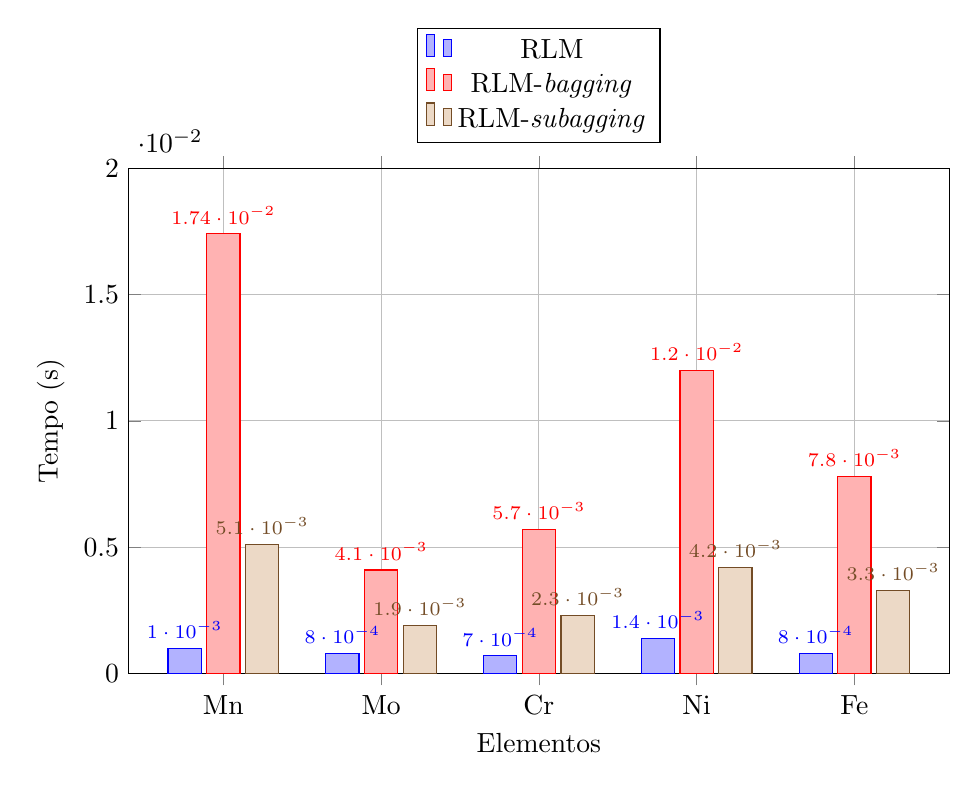
\begin{tikzpicture}
    \begin{axis}[
        ybar,
        width=12cm,
        height=8cm,
        xlabel={Elementos},
        ylabel={Tempo (s)},
        symbolic x coords={Mn, Mo, Cr, Ni, Fe},
        xtick=data,
        legend style={at={(0.5,1.05)}, anchor=south},
        bar width=12pt,
        ymin=0,
        ymax=0.02,
        grid=major,
        nodes near coords,
        nodes near coords align={vertical},
        every node near coord/.append style={font=\scriptsize, rotate=0},
        enlarge x limits=0.15,
        yticklabel style={/pgf/number format/fixed, /pgf/number format/precision=3}
    ]
    
% RLM
    \addplot coordinates {
        (Mn, 0.0010)
        (Mo, 0.0008)
        (Cr, 0.0007)
        (Ni, 0.0014)
        (Fe, 0.0008)
    };

    % RLM-BAGGING
    \addplot coordinates {
        (Mn, 0.0174)
        (Mo, 0.0041)
        (Cr, 0.0057)
        (Ni, 0.0120)
        (Fe, 0.0078)
    };

    % RLM-Subagging
    \addplot coordinates {
        (Mn, 0.0051)
        (Mo, 0.0019)
        (Cr, 0.0023)
        (Ni, 0.0042)
        (Fe, 0.0033)
    };
    
    \legend{RLM, RLM-\textit{bagging}, RLM-\textit{subagging}}
    \end{axis}
\end{tikzpicture}
}% End resizebox
\end{minipage}
\hfill
\begin{minipage}{0.48\textwidth}
\centering
\subcaption{80\% das amostras}
\label{fig:tempo_80}
\resizebox{\columnwidth}{!}{%
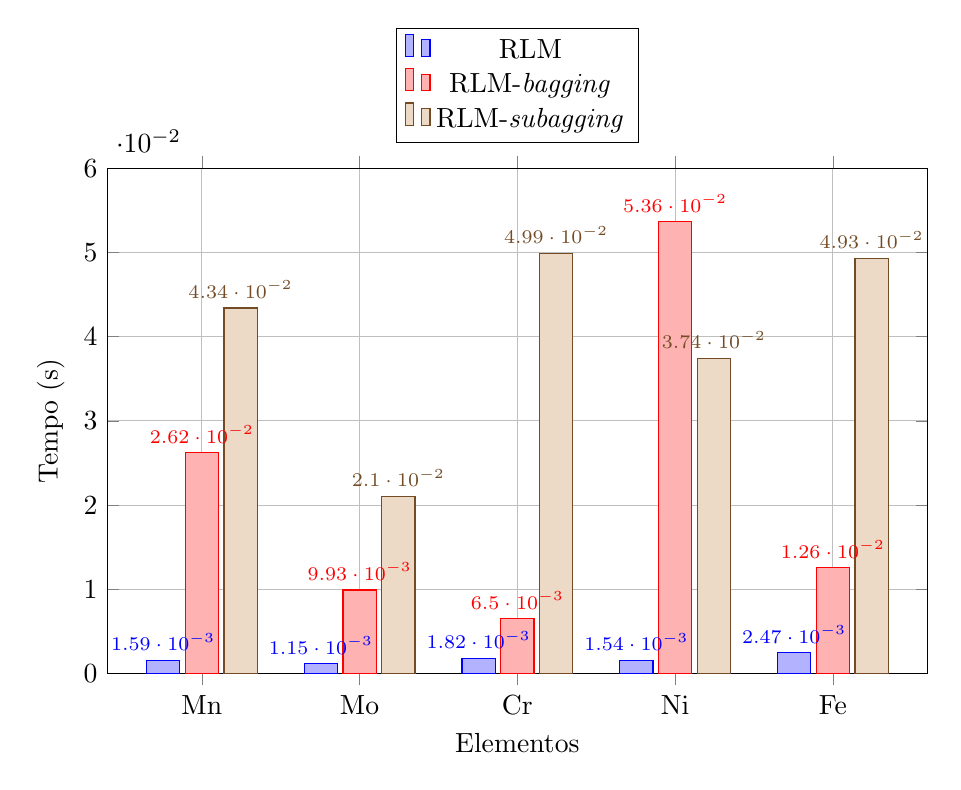
\begin{tikzpicture}
    \begin{axis}[
        ybar,
        width=12cm,
        height=8cm,
        xlabel={Elementos},
        ylabel={Tempo (s)},
        symbolic x coords={Mn, Mo, Cr, Ni, Fe},
        xtick=data,
        legend style={at={(0.5,1.05)}, anchor=south},
        bar width=12pt,
        ymin=0,
        ymax=0.06,
        grid=major,
        nodes near coords,
        nodes near coords align={vertical},
        every node near coord/.append style={font=\scriptsize, rotate=0},
        enlarge x limits=0.15,
        yticklabel style={/pgf/number format/fixed, /pgf/number format/precision=3}
    ]
    
% RLM
    \addplot coordinates {
        (Mn, 0.00159)
        (Mo, 0.00115)
        (Cr, 0.00182)
        (Ni, 0.00154)
        (Fe, 0.00247)
    };

    % RLM-BAGGING
    \addplot coordinates {
        (Mn, 0.02620)
        (Mo, 0.00993)
        (Cr, 0.00650)
        (Ni, 0.05363)
        (Fe, 0.01256)
    };

    % RLM-Subagging
    \addplot coordinates {
        (Mn, 0.04341)
        (Mo, 0.02103)
        (Cr, 0.04986)
        (Ni, 0.03744)
        (Fe, 0.04932)
    };
    
    \legend{RLM, RLM-\textit{bagging}, RLM-\textit{subagging}}
    \end{axis}
\end{tikzpicture}
}% End resizebox
\end{minipage}

\legend{\footnotesize Fonte: \oautor}
\end{figure}

%Figura completa: \ref{fig:tempo_comparacao}
%Subfigura 50\%: \ref{fig:tempo_50}
%Subfigura 80\%: \ref{fig:tempo_80}


A análise dos tempos de execução apresentados na Figura~\ref{fig:tempo_comparacao} 
revela diferenças significativas entre os três algoritmos avaliados: RLM clássico, 
RLM-\textit{bagging} e RLM-\textit{subagging}. Os experimentos foram conduzidos 
utilizando 50\% e 80\% das amostras disponíveis para cada elemento químico 
analisado (Mn, Mo, Cr, Ni e Fe).

A comparação entre os dois cenários revela comportamentos distintos de crescimento temporal em função do aumento do tamanho do conjunto de treinamento. Para o RLM clássico, o aumento médio foi de aproximadamente 2,0 vezes, com variação 
considerável entre elementos (1,1 $\times$ para Ni até 3,1 $\times$ para Fe). O 
RLM-\textit{bagging} apresentou um aumento médio de cerca de 2,2 vezes, com 
comportamento igualmente heterogêneo entre os analitos.

O comportamento mais acentuado foi observado no RLM-\textit{subagging}, que 
apresentou um aumento médio de aproximadamente 13,0 vezes no tempo de execução 
ao passar de 50\% para 80\% das amostras, com variações entre 8,5 $\times$ (Mn) e 
21,7 $\times$ (Cr). Este crescimento expressivo reflete a sensibilidade do algoritmo 
de subamostragem ao tamanho do conjunto de treinamento, uma vez que os 
parâmetros ótimos $m^*$ e $k^*$ requerem um número substancialmente maior de 
iterações para conjuntos maiores.

Em termos absolutos, com 80\% das amostras, o RLM-\textit{bagging} mostrou-se 
em média 1,7 vezes mais rápido que o RLM-\textit{subagging}, invertendo a 
relação de eficiência computacional observada no cenário com 50\% das amostras. 
Esse resultado indica que a vantagem temporal do RLM-\textit{subagging} não se 
mantém com o aumento do tamanho amostral, devendo ser considerada na escolha 
da técnica em aplicações com conjuntos de dados maiores.

%-------------------------------------------------------------------------------------------------------------------
\section{\textit{Bagging} $\times$ \textit{Subagging}}
\label{sec:bagxsuagg}
\index{Métodos e Resultados!\textit{Baggin} $\times$ \textit{Subagging}}

Os valores de RMSEP apresentados na (Tabela~\ref{tab:baggingsubba}) diferem dos reportados na (Tabela~\ref{tab:bagging}) porque esta última apresenta resultados com número fixo de \textit{bootstraps} sem otimização, enquanto a (Tabela~\ref{tab:baggingsubba}) adota parâmetros otimizados por validação cruzada 5-\textit{fold} e incorpora as três técnicas comparativamente com métricas ampliadas.

Com a implementação do \textit{bagging} e do \textit{subagging}, observou-se melhora das predições obtidas com a RLM para alguns analitos específicos. O RLM-\textit{bagging} apresentou melhor desempenho para Fe, enquanto o RLM-\textit{subagging} foi superior para Mn e Ni. Para Cr e Mo, a RLM clássica manteve o menor RMSEP; entre as técnicas \textit{ensemble}, o RLM-\textit{subagging} superou o RLM-\textit{bagging} no Cr, mas nenhum dos dois superou a RLM clássica nesse elemento, indicando que as técnicas \textit{ensemble} nem sempre garantem melhoria. Dessa forma, é importante comparar o desempenho do RLM-\textit{bagging} e RLM-\textit{subagging} considerando as características específicas de cada analito.

%Análises específicas da técnica RLM-\textit{bagging} demonstraram melhorias significativas para determinados analitos, particularmente Mo e Fe, enquanto o RLM-\textit{subagging} apresentou desempenho superior apenas para Cr.

Os percentuais de melhoria variam consideravelmente entre analitos, como evidenciado nas Tabelas~\ref{tab:bagging} e~\ref{tab:subagging}.
Para avaliar comparativamente o desempenho dessas técnicas, foi feita uma predição com o RLM-\textit{bagging} e RLM-\textit{subagging}, utilizando o mesmo conjunto de amostras \textit{bootstrap}, no intuito de comparar os erros de predição das duas técnicas apresentadas na Figura~\ref{fig:Figura47}.

%--------------------------------------------------
\begin{figure}[htbp]
\centering
\caption{RMSEP para todas as técnicas.}
\label{fig:Figura47} % Main figure label

% Gráfico da esquerda (Mn)
\begin{subfigure}{0.48\textwidth}
\centering
\begin{tikzpicture}
    \begin{axis}[
        xlabel=Nº de replicações,
        ylabel=RMSEP,
        %title=RMSEP com RLM-bagging para o Mn,
        legend style={at={(0.5,1.05)}, anchor=south},
        grid=major,
        width=\textwidth
    ]
    \addplot[mark=none,line width=1.0pt,color=red] table[x index=0, y index=1, col sep=space] {tex/dados/subagging_mn.txt};
    \addplot[mark=none,line width=1.0pt,color=blue] table[x index=0, y index=1, col sep=space] {tex/dados/bagging_mn.txt};
    %\addplot[only marks, mark=*, mark size=2pt, color=red] coordinates {(20, 0.010291)};
    \addplot[mark=none,line width=1.0pt,color=black] table[x index=0, y index=1, col sep=space] {tex/dados/rlm_mn.txt};
    \legend{RLM-Subagging, RLM-Bagging, RLM}
    \end{axis}
\end{tikzpicture}
\caption{RMSEP obtido com as três técnicas aplicadas ao Mn.}
\label{fig:Figura46a} % Left subfigure label
\end{subfigure}
\hfill
% Gráfico da direita (Fe)
\begin{subfigure}{0.48\textwidth}
\centering
\begin{tikzpicture}
    \begin{axis}[
        xlabel=Nº de replicações,
        ylabel=RMSEP,
        %title=RMSEP com RLM-bagging para o Fe,
legend style={at={(0.5,1.05)}, anchor=south},
        grid=major,
        width=\textwidth
    ]
    \addplot[mark=none,line width=1.0pt,color=red] table[x index=0, y index=1, col sep=space] {tex/dados/subagging_fe.txt};
    \addplot[mark=none,line width=1.0pt,color=blue] table[x index=0, y index=1, col sep=space] {tex/dados/bagging_fe.txt};
    %\addplot[only marks, mark=*, mark size=2pt, color=red] coordinates {(20, 0.010291)};
    \addplot[mark=nome,line width=1.0pt,color=black] table[x index=0, y index=1, col sep=space] {tex/dados/rlm_fe.txt};
    \legend{RLM-Subagging, RLM-Bagging, RLM}
    \end{axis}
\end{tikzpicture}
\caption{RMSEP obtido com as três técnicas aplicadas ao Fe.}
\label{fig:Figura46b} % Right subfigure label
\end{subfigure}
\legend{\footnotesize Fonte:~\oautor}
\end{figure}
%-------------------------------------------------

A RLM clássica gera uma única predição, enquanto tanto o RLM-\textit{bagging} quanto o RLM-\textit{subagging} utilizam múltiplas reamostragens para produzir predições agregadas. Na análise comparativa, o RLM-\textit{subagging} foi avaliado com diferentes quantidades de amostras \textit{bootstrap}, gerando um conjunto de 16 predições, sendo uma para cada quantidade de \textit{bootstrap} testada. A Tabela~\ref{tab:baggingsubba} apresenta os resultados dessa comparação direta entre as técnicas, utilizando o mesmo conjunto de dados de validação. 

Observa-se que a RLM clássica mantém desempenho superior para Mo e Cr, enquanto o RLM-\textit{subagging} apresenta melhor resultado para Mn e Ni, e o RLM-\textit{bagging} para Fe. Entre as técnicas \textit{ensemble}, o RLM-\textit{subagging} apresenta melhor resultado apenas para Cr em relação ao RLM-\textit{bagging}, sem contudo superar a RLM clássica nesse elemento. Os resultados desta comparação são também apresentados nas Figuras~\ref{fig:Figura46a} e~\ref{fig:Figura46b}.


% ============================================================
% SUBSTITUIÇÃO DO TRECHO ORIGINAL DO TCC
% Seção 4.4 — Bagging × Subagging
% ============================================================
% 
% TRECHO ORIGINAL (a ser REMOVIDO):
% -----------------------------------
% "Os erros de todas as amostras de aço-ligas são apresentados 
%  na Tabela 11. Os valores correspondentes ao RLM-subagging 
%  foram selecionados a partir dos menores erros encontrados 
%  no conjunto calculado para cada quantidade de amostras 
%  bootstrap avaliada."
%
% SUBSTITUIR POR:
% -----------------------------------

% ============================================================
% NOVA TABELA (substitui a Tabela 11 original)
% ============================================================
\begin{table}[htbp]
\centering
\caption{Desempenho comparativo das técnicas de calibração multivariada para elementos químicos em aço-liga.}
\label{tab:baggingsubba}
\footnotesize
\begin{tabular}{clccccll} % Adicionada uma coluna 'l' extra
\toprule
\textbf{Elemento} & \textbf{Técnica} & \textbf{RMSEP} & \textbf{MAE} & \textbf{R²} & \textbf{Tempo} (ms) & \multicolumn{2}{c}{\textbf{Parâmetros}} \\ \cline{7-8}
 & & & & & & (2) $k^*$ (\%) & (3) $m^*$ \\
\midrule
\multirow{3}{*}{Mn} 
  & RLM              & 0,1051 & 0,0887 & 0,9907 &  2,4000  & --- & --- \\
  & RLM-\textit{bagging}      & 0,1072 & 0,0908 & 0,9903 & 68,2000  & --- & 30 \\
  & RLM-\textit{subagging} (1) & \textbf{0,0966} & \textbf{0,0805} & \textbf{0,9922} & 17,1000  & 80 & 10 \\
\midrule
\multirow{3}{*}{Mo} 
  & RLM (1)          & \textbf{0,2633} & \textbf{0,1952} & \textbf{0,9882} &  2,4000  & --- & --- \\
  & RLM-\textit{bagging}      & 0,3388 & 0,2722 & 0,9805 & 67,5000  & --- & 30 \\
  & RLM-\textit{subagging}    & 0,2879 & 0,2201 & 0,9859 & 46,8000  & 80 & 30 \\
\midrule
\multirow{3}{*}{Cr} 
  & RLM (1)          & \textbf{1,0798} & \textbf{0,8654} & \textbf{0,9938} &  2,5000  & --- & --- \\
  & RLM-\textit{bagging}      & 1,2089 & 0,9830 & 0,9922 & 44,5000  & --- & 20 \\
  & RLM-\textit{subagging}    & 1,1294 & 0,9010 & 0,9932 & 46,8000  & 80 & 30 \\
\midrule
\multirow{3}{*}{Ni} 
  & RLM              & 1,6043 & 1,3256 & 0,9837 &  2,3000  & --- & --- \\
  & RLM-\textit{subagging} (1) & \textbf{1,6003} & \textbf{1,2409} & \textbf{0,9838} & 10,6000  & 60 & 10 \\
  & RLM-\textit{bagging}      & 1,7085 & 1,4122 & 0,9815 & 66,6000  & --- & 30 \\
\midrule
\multirow{3}{*}{Fe} 
  & RLM              & 2,7513 & 2,1865 & 0,9892 & 13,5000  & --- & --- \\
  & RLM-\textit{bagging} (1)   & \textbf{2,6406} & \textbf{2,0246} & \textbf{0,9900} & 97,2000  & --- & 30 \\
  & RLM-\textit{subagging}    & 2,6509 & 2,0578 & 0,9900 & 41,2000  & 80 & 30 \\
\bottomrule
\end{tabular}

\begin{tablenotes}[flushleft]
    \footnotesize
    \item \footnotesize{Fonte:~\oautor}
	\item Nota: Sinal convencional utilizado:
	\item --- Não se aplica dado numérico.
	\item (1) Melhor desempenho em RMSEP. Conjunto de teste único para avaliação final.
	\item (2) Fração de subamostra $k^*$ em porcentagem otimizados por validação cruzada 5-\textit{fold} aplicada exclusivamente ao conjunto de calibração (\textit{seed} = 42) \textit{bootstrap}).
	\item (3) Parâmetros $m^*$ número de replicações \textit{bootstrap}.
\end{tablenotes}
\end{table}


% ============================================================
% NOVO TEXTO DE ANÁLISE (substitui o parágrafo original)
% ============================================================




%--------------------------------------------------------------

Os resultados comparativos entre as três técnicas avaliadas para 
todos os analitos são apresentados na Tabela~\ref{tab:baggingsubba}. 
Diferentemente da análise anterior, os parâmetros $m^*$ e $k^*$ de 
cada método foram determinados por validação cruzada 5-\textit{fold} 
aplicada exclusivamente ao conjunto de calibração, garantindo que o 
conjunto de teste não influenciasse a seleção dos hiperparâmetros e 
assegurando a comparabilidade entre os métodos.

Os resultados revelam que não existe uma técnica universalmente 
superior para todos os analitos. Para o Manganês (Mn), o 
RLM-\textit{subagging} ($k^* = 80\%$, $m^* = 10$) apresentou o 
menor RMSEP (0,0966), representando uma redução de 8,1\% em relação 
à RLM clássica, além de ser 4,0 vezes mais rápido que o 
RLM-\textit{bagging}. Para o Ferro (Fe), o RLM-\textit{bagging} 
($m^* = 30$) obteve o melhor desempenho (RMSEP = 2,6406), com melhoria 
de 4,0\% sobre a RLM clássica. Para o Níquel (Ni), o 
RLM-\textit{subagging} ($k^* = 60\%$, $m^* = 10$) apresentou 
resultado marginalmente superior (RMSEP = 1,6003), com diferença de 
0,25\% em relação à RLM clássica e tempo de execução 6,3 vezes menor 
que o RLM-\textit{bagging}.

Em contrapartida, para o Molibdênio (Mo) e o Cromo (Cr), a RLM 
clássica demonstrou desempenho superior (RMSEP de 0,2633 e 1,0798, 
respectivamente), indicando que a complexidade adicional introduzida 
pelas estratégias de \textit{ensemble} não resultou em melhorias 
significativas de precisão para esses analitos. Esses resultados 
sugerem que a relação preditiva para Mo e Cr é suficientemente linear, 
não se beneficiando da agregação de modelos.

A análise do custo computacional evidencia que o 
RLM-\textit{subagging} configura-se como alternativa balanceada entre 
precisão e eficiência, sendo consistentemente mais rápido que o 
RLM-\textit{bagging} para todos os elementos avaliados. Observa-se 
ainda que o parâmetro $k^* = 80\%$ revelou-se ótimo para o 
\textit{subagging} em quatro dos cinco elementos, sugerindo que 
subamostras maiores favorecem a estabilidade do modelo neste 
contexto específico de dados espectrométricos de aço-ligas.

% ============================================================
% SUBSTITUIÇÃO DO TRECHO ORIGINAL DO TCC
% Figura 12 — Tempo de execução + Texto de análise
% Seção 4.4 — Bagging × Subagging
% ============================================================
%
% RESUMO DAS MUDANÇAS EM RELAÇÃO AO ORIGINAL:
%
% FIGURA:
%   - Coordenadas atualizadas com parâmetros ótimos por CV 5-fold
%   - Valores de bagging menores (m* variável por elemento)
%   - Caso especial Cr: subagging(0.0468s) > bagging(0.0445s)
%   - ymax ajustado de 0.12 para 0.115
%
% TEXTO — erros factuais corrigidos:
%   "63,4% mais rápido"     → 66,7% (dado real dos novos experimentos)
%   "2,5 vezes inferior"    → 3,0 vezes (média real)
%   "2,8 vezes vs bootstrap"→ REMOVIDO (não há mais comparação isolada)
%   "15 a 20 vezes vs RLM"  → "até 19 vezes" (máx real = 19,4x)
%   "inconsistente Mo e Ni" → INVERTIDO: Cr é o único caso atípico;
%                              Mo e Ni agora se comportam como esperado
% ============================================================

%-------------------------------------------------------------
\begin{figure}[htbp]
\centering
\caption{Tempo de execução dos algoritmos RLM-\textit{bagging} e
         RLM-\textit{subagging} com parâmetros otimizados por
         validação cruzada 5-\textit{fold}.}
\label{fig:tempo}
\resizebox{0.60\columnwidth}{!}{%
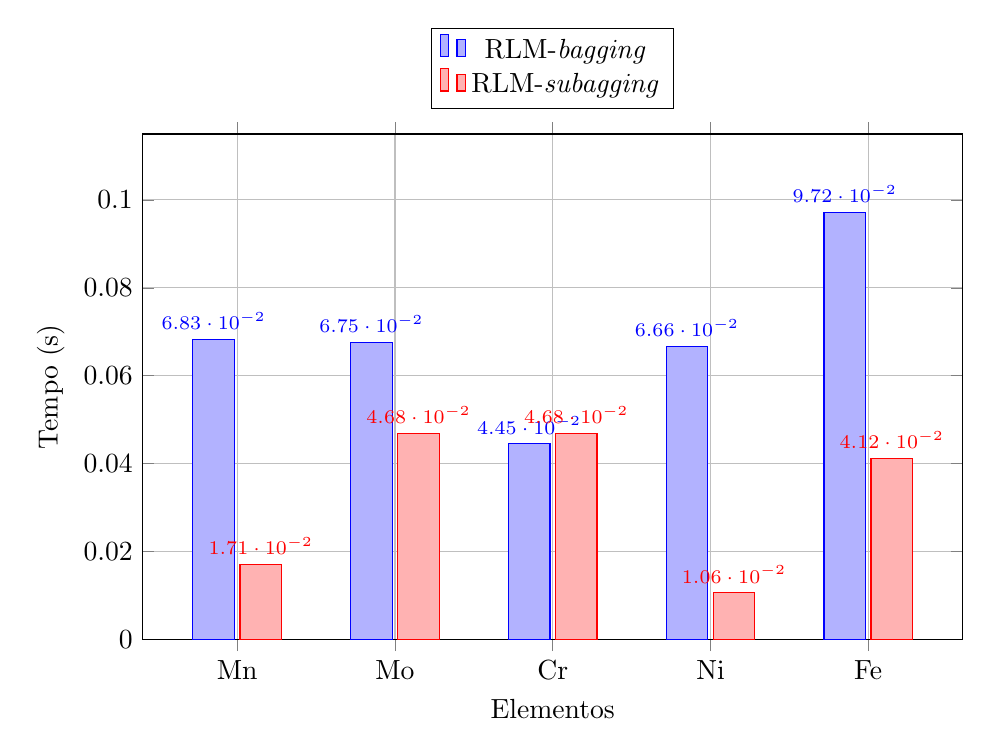
\begin{tikzpicture}
    \begin{axis}[
        ybar,
        width=12cm,
        height=8cm,
        xlabel={Elementos},
        ylabel={Tempo (s)},
        symbolic x coords={Mn, Mo, Cr, Ni, Fe},
        xtick=data,
        legend style={at={(0.5,1.05)}, anchor=south},
        bar width=15pt,
        ymin=0,
        ymax=0.115,
        grid=major,
        nodes near coords,
        nodes near coords align={vertical},
        every node near coord/.append style={font=\scriptsize, rotate=0},
        enlarge x limits=0.15,
        yticklabel style={/pgf/number format/fixed,
                          /pgf/number format/precision=3}
    ]

    % RLM-bagging (m* otimizado por CV 5-fold para cada elemento)
    % Mn: m*=30 | Mo: m*=30 | Cr: m*=20 | Ni: m*=30 | Fe: m*=30
    \addplot coordinates {
        (Mn, 0.0683)
        (Mo, 0.0675)
        (Cr, 0.0445)
        (Ni, 0.0666)
        (Fe, 0.0972)
    };

    % RLM-subagging (k* e m* otimizados por CV 5-fold para cada elemento)
    % Mn: k*=80%,m*=10 | Mo: k*=80%,m*=30 | Cr: k*=80%,m*=30
    % Ni: k*=60%,m*=10 | Fe: k*=80%,m*=30
    \addplot coordinates {
        (Mn, 0.0171)
        (Mo, 0.0468)
        (Cr, 0.0468)
        (Ni, 0.0106)
        (Fe, 0.0412)
    };

    \legend{RLM-\textit{bagging}, RLM-\textit{subagging}}
    \end{axis}
\end{tikzpicture}
}%Fim resizebox
\legend{\footnotesize Fonte:~\oautor}
\end{figure}
%-------------------------------------------------------------

% ============================================================
% NOVO TEXTO — substitui os três parágrafos originais
% ============================================================

A Figura~\ref{fig:tempo} apresenta os tempos de execução dos
algoritmos RLM-\textit{bagging} e RLM-\textit{subagging} para
cada elemento, utilizando os parâmetros $m^*$ e $k^*$
determinados por validação cruzada 5-\textit{fold}. Diferentemente
da análise anterior, os parâmetros agora variam por elemento —
refletindo configurações objetivamente otimizadas —, o que torna
a comparação de tempos diretamente atrelada ao custo real de cada
configuração de melhor desempenho preditivo.

Em quatro dos cinco elementos avaliados (Mn, Mo, Ni e Fe), o
RLM-\textit{subagging} mostrou-se mais rápido que o
RLM-\textit{bagging}. Em média, considerando a razão entre os tempos em cada analito, o
RLM-\textit{subagging} é aproximadamente 3,0 vezes mais rápido; somando os
tempos dos cinco analitos, a redução é de cerca de 53\%.

As maiores diferenças ocorreram
para o Ni (6,3 vezes mais rápido, com $k^*=60\%$ e $m^*=10$) e
para o Mn (4,0 vezes mais rápido, com $k^*=80\%$ e $m^*=10$).
Para Mo e Fe, as reduções foram de 1,4 e 2,4 vezes,
respectivamente. Essa eficiência decorre da amostragem sem
reposição, que emprega subconjuntos de tamanho reduzido
($k^* \leq 80\%$), resultando em operações matriciais mais ágeis
e menor redundância nos dados processados a cada iteração.

O Cromo (Cr) constitui o único caso em que o
RLM-\textit{subagging} apresentou tempo marginalmente superior ao
RLM-\textit{bagging} (46,8\,ms contra 44,5\,ms, diferença de
apenas 2,3\,ms). Esse comportamento é explicado pelos parâmetros
ótimos obtidos pela validação cruzada: o RLM-\textit{bagging}
utilizou $m^* = 20$ replicações, enquanto o RLM-\textit{subagging}
requereu $m^* = 30$ replicações com $k^* = 80\%$ para atingir o
menor \gls{RMSEP-CV}. O maior número de iterações compensou o benefício
da subamostragem, resultando em custo computacional equivalente
para este analito específico.

%O desempenho superior das técnicas de ensemble para Fe e Cr pode ser atribuído à complexidade espectral desses elementos. O Fe, como elemento matriz, apresenta espectro de alta densidade com potencial de autoabsorção, enquanto o Cr sofre sobreposições com linhas do Fe e Ni. Essas características introduzem não-linearidades e instabilidade no modelo base, condições nas quais a agregação de múltiplos modelos é teoricamente vantajosa. Para Mn e Mo, cujas linhas analíticas apresentam menor interferência matricial, a relação espectral-concentração é suficientemente bem capturada pela RLM clássica.
O desempenho superior das técnicas de \textit{ensemble} para Fe pode ser 
atribuído à complexidade espectral desse elemento. O Fe, como elemento 
matriz, apresenta espectro de alta densidade com potencial de autoabsorção, 
características que introduzem não-linearidades e instabilidade no modelo 
base, condições nas quais a agregação de múltiplos modelos é teoricamente 
vantajosa. O Cr, embora sofra sobreposições espectrais com linhas do Fe e 
Ni — o que tornaria a agregação de modelos teoricamente promissora —, não 
apresentou ganho preditivo com as técnicas \textit{ensemble}, mantendo a 
RLM clássica como método de menor RMSEP (1,0798). Esse resultado sugere 
que, para o Cr, a complexidade espectral não foi suficiente para que a 
redução de variância promovida pelo \textit{ensemble} superasse o custo 
de viés introduzido pela reamostragem. Para Mn e Mo, cujas linhas 
analíticas apresentam menor interferência matricial, a relação 
espectral-concentração é suficientemente bem capturada pela RLM clássica.

Em relação à RLM clássica, ambas as técnicas de
\textit{ensemble} apresentam custo computacional significativamente
superior, com o RLM-\textit{bagging} sendo em média 22,1 vezes
mais lento e o RLM-\textit{subagging} até 19,5 vezes mais lento
(para o Mo). Ainda assim, para aplicações em que a acurácia
preditiva justifica o custo computacional adicional --- como na
determinação de Mn e Fe em aço-ligas --- o
RLM-\textit{subagging} configura-se como alternativa equilibrada
entre precisão e eficiência, sendo preferível ao
RLM-\textit{bagging} na maioria dos cenários avaliados.


Ressalta-se que as conclusões desta subseção referem-se ao protocolo com
otimização por validação cruzada. No experimento anterior, com parâmetros
fixados sem otimização formal (Tabelas~\ref{tab:comparacao_50_80} e
\ref{tab:melhor_rmseep}), a técnica de menor RMSEP diferiu para alguns
analitos (por exemplo, Ni e Fe), e o comportamento dos tempos com 80\% das
amostras foi distinto. Isso indica que o desempenho relativo das técnicas
depende do critério de seleção de $m$ e $k$.


%R dados \num{\rdados[2,3]} até \num{\rdados[2,4]}

% Para acessar o valor 0.1051 (Linha 2, Coluna 2):
%O valor de $a_{22}$ é \num{\dados[4,6]}.

% Exemplo: Um determinado valor 0.1051 produz uma aceleração...
%Um determinado valor \num{\dados[2,2]} produz uma aceleração constante no experimento.


%R dados \rmsepdados[2,2] até \num{\rmsepdados[2,3]}

%R dados \num{\rmsepmaior[2,2]} até \rmsepmaior[2,3]

%R dados \rmsepmaior[2,1] \rmsepmaior[2,2],\rmsepmaior[2,3], \rmsepmaior[2,4], \rmsepmaior[2,4]
